\documentclass[10pt,a4paper]{article}
\usepackage[margin=2cm]{geometry}
\usepackage{amsmath,amssymb,booktabs,graphicx,caption,subcaption,xcolor,float,hyperref,tikz}
\usetikzlibrary{arrows.meta,positioning,fit,calc}
\hypersetup{colorlinks=true,linkcolor=blue!50!black,urlcolor=blue!50!black}
\captionsetup{font=small,labelfont=bf}
\newcounter{diagram}
\newcommand{\diagramcaption}[1]{\refstepcounter{diagram}\par\smallskip\noindent{\small\textbf{Diagram~\thediagram.} #1}}
\title{\vspace{-1.2cm}\textbf{A swarm that owns a proof can still lose it}\\[2pt]
\large Simulation 1, setup \texttt{task003-symmetric}: first results}
\author{LLM-free simulator, runs of 7 October 2026}
\date{}
\begin{document}
\maketitle
\vspace{-1cm}

\paragraph{Summary.} 24 agents together hold a complete proof that allocation A0 is
correct, but no single agent does. A controller steers toward A0 (truth) or A2
(false). (i)~\textbf{Whether the false controller wins depends on memory}: when agents
forget, it overturns the proof; with full memory its success is temporary, because its
own true facts end up completing proofs of A0. (ii)~\textbf{The controller senses the
swarm accurately}, so its failures are not sensing failures. (iii)~\textbf{Helping the
truth is not the same as helping agents assemble their own proof}: extra truth posts
raise the share of agents holding a proof, but lower the share holding one from their
own evidence.

\section{Setup}

\begin{center}
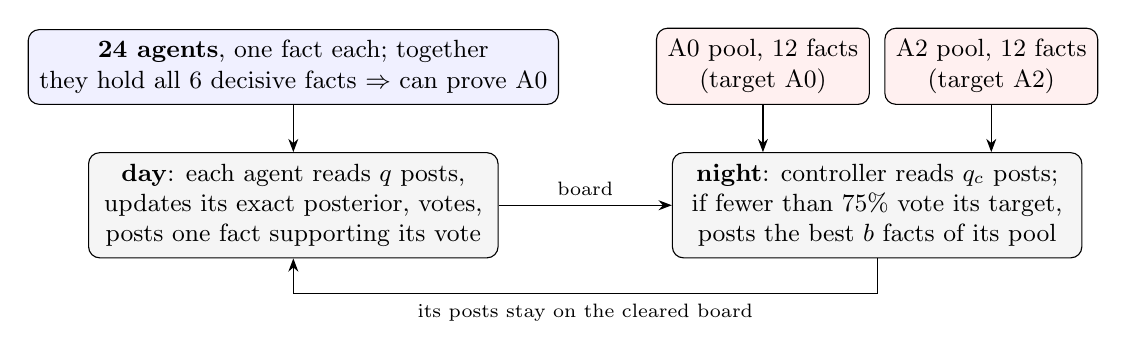
\begin{tikzpicture}[font=\small, box/.style={draw, rounded corners, align=center, inner sep=4pt}]
  \node[box, fill=gray!8, minimum width=5.2cm] (day) {\textbf{day}: each agent reads $q$ posts,\\
     updates its exact posterior, votes,\\ posts one fact supporting its vote};
  \node[box, fill=gray!8, right=2.2cm of day, minimum width=5.2cm] (night) {\textbf{night}: controller reads $q_c$ posts;\\
     if fewer than 75\% vote its target,\\ posts the best $b$ facts of its pool};
  \node[box, fill=blue!6, above=0.6cm of day, minimum width=5.2cm] (agents) {\textbf{24 agents}, one fact each; together\\
     they hold all 6 decisive facts $\Rightarrow$ can prove A0};
  \node[box, fill=red!6, above=0.6cm of night, xshift=-1.45cm] (p0) {A0 pool, 12 facts\\ (target A0)};
  \node[box, fill=red!6, above=0.6cm of night, xshift=1.45cm] (p2) {A2 pool, 12 facts\\ (target A2)};
  \draw[-{Stealth}] (agents) -- (day);
  \draw[-{Stealth}] (p0) -- (p0 |- night.north);
  \draw[-{Stealth}] (p2) -- (p2 |- night.north);
  \draw[-{Stealth}] (day) -- node[above, font=\scriptsize]{board} (night);
  \draw[-{Stealth}] (night.south) -- ++(0,-0.45) -| node[below, pos=0.25, font=\scriptsize]{its posts stay on the cleared board} (day.south);
\end{tikzpicture}
\diagramcaption{One round of Simulation 1: a day followed by a night, repeated for 30
rounds. Each dawn, every remembered fact survives with probability $\rho$.}
\label{dia:setup}
\end{center}

The two pools share no fact, contain no decisive fact, cannot prove their target, and
are matched in strength pair by pair. The agents start, in expectation, with 9 / 7 / 8
votes for A0 / A1 / A2. Agents are exact Bayesian reasoners: an agent's belief is the
exact posterior over the three allocations given the facts it remembers. Three agent
rules are compared: \emph{argmax} voting with posts that support the vote (the
\emph{base} rule), \emph{probability matching} (vote drawn from the posterior), and
argmax with \emph{uniform} posts (a random remembered fact, whatever the vote).

\paragraph{Measuring control.} Every episode is run three times with the same random
draws: silent, truth controller, false controller. The \emph{paired gain} of a
controller in the share of agents voting for allocation $a$ on day $t$ is
\begin{equation}\label{eq:gain}
G_t^{(a)} = \frac{1}{E}\sum_{e=1}^{E}\Bigl[x_{a,t}^{\text{ctrl}}(e) - x_{a,t}^{\text{silent}}(e)\Bigr],
\end{equation}
with $E = 1000$ episodes per cell and 95\% intervals from resampling episodes.

\section{A swarm that owns a proof can still lose it}

\begin{figure}[H]
\centering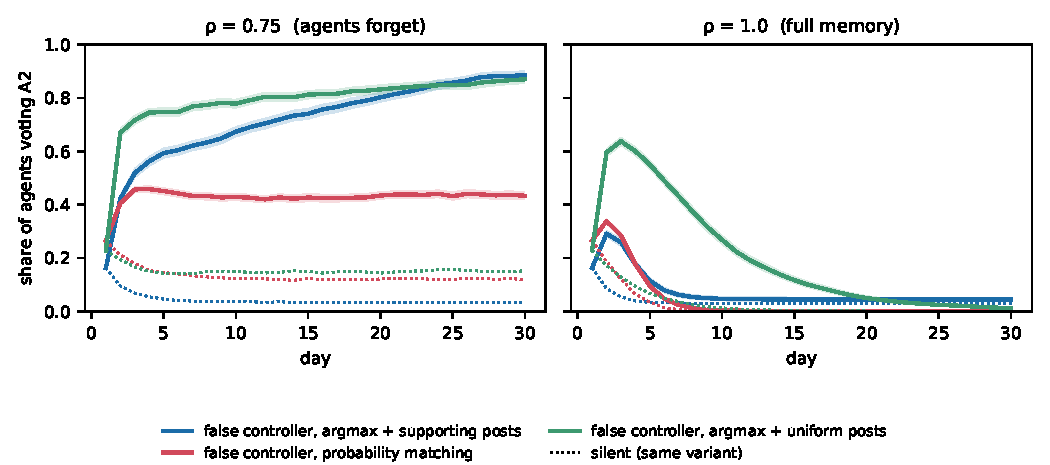
\includegraphics[width=0.95\linewidth]{figures/fig_a2_share_time.pdf}
\caption{Share of agents voting A2 over the days, under the false controller (solid,
95\% band) and without a controller (dotted). $q = 6$, $q_c = 12$, $b = 3$.}
\label{fig:a2time}
\end{figure}

Figure~\ref{fig:a2time} shows the central result. \textbf{When agents forget}
($\rho = 0.75$), the false controller pushes the A2 share from under 0.2 to about 0.9
under the base and uniform rules, and to about 0.45 under probability matching.
\textbf{With full memory} ($\rho = 1$) every rule shows the same shape: an early A2
peak (up to 0.6 under uniform posts), then a return to A0 by day 20. Table~\ref{tab:gain}
gives the day-30 gains.

\begin{table}[H]
\centering\small
\caption{Day-30 paired gain of the false controller in the A2 share, Eq.~(\ref{eq:gain});
$q_c = 12$, $b = 3$.}
\label{tab:gain}
\begin{tabular}{llccc}
\toprule
$\rho$ & agent rule & $q = 3$ & $q = 6$ & $q = 12$ \\
\midrule
0.75 & argmax + supporting posts & 0.95 & 0.85 & 0.26 \\
0.75 & probability matching & 0.48 & 0.32 & 0.08 \\
0.75 & argmax + uniform posts & 0.67 & 0.72 & 0.69 \\
\midrule
1.0 & argmax + supporting posts & 0.03 & 0.01 & 0.00 \\
1.0 & probability matching & 0.00 & 0.00 & 0.00 \\
1.0 & argmax + uniform posts & 0.05 & 0.01 & 0.01 \\
\bottomrule
\end{tabular}
\end{table}

\begin{figure}[H]
\centering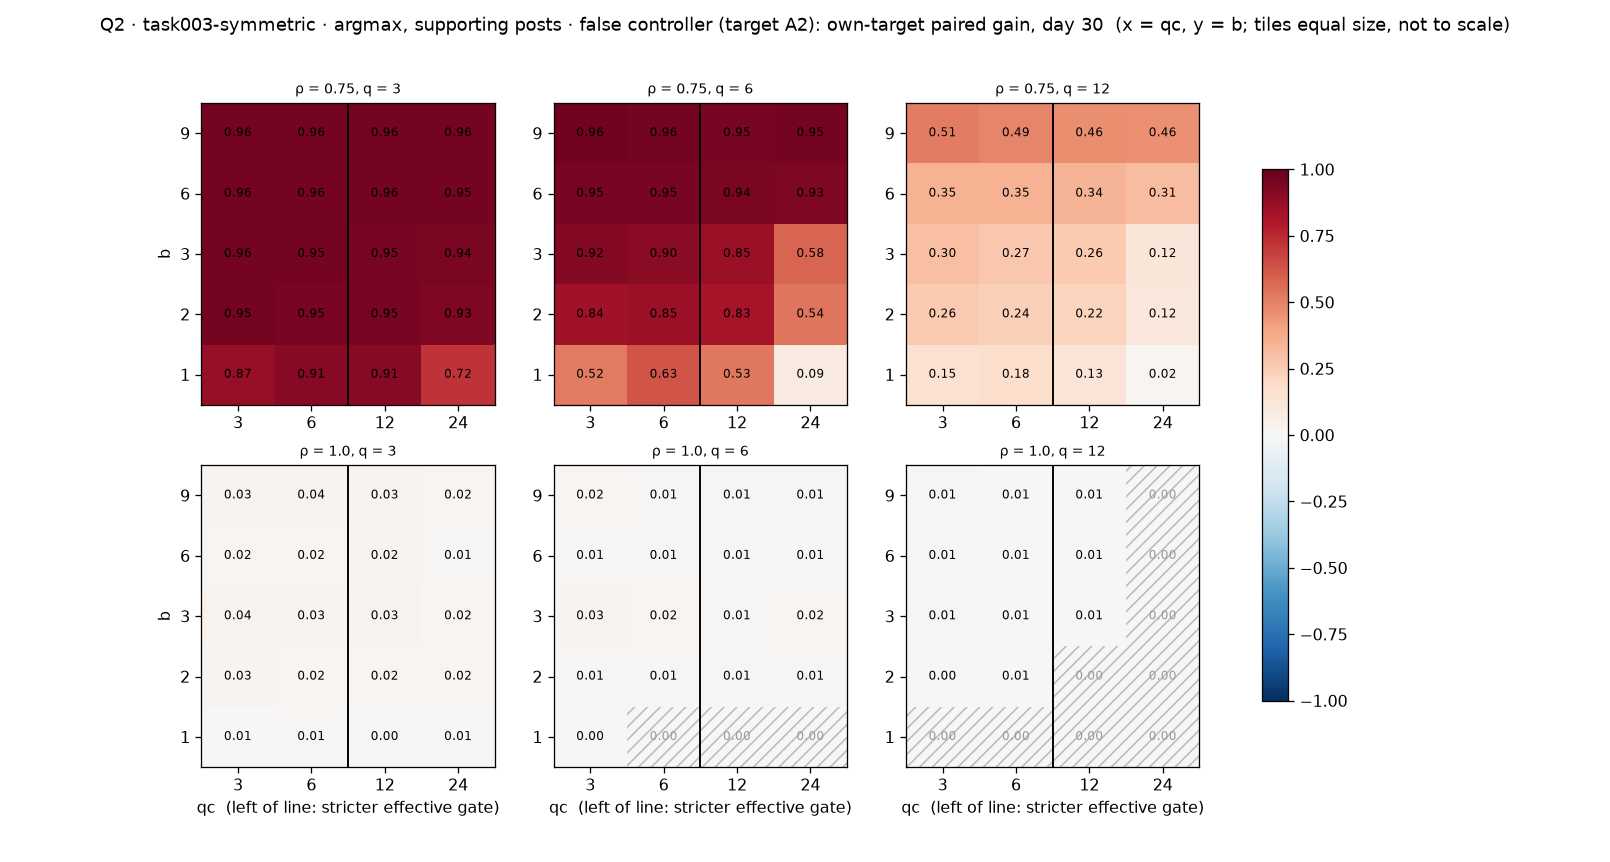
\includegraphics[width=0.92\linewidth]{figures/phase_false_base.png}
\caption{Day-30 paired gain of the false controller (A2 share) over the reading budget
$q_c$ (x) and posting budget $b$ (y); base rule. Rows: $\rho$; columns: $q$. Tiles are
equal size, not to scale. Left of the black line, the vote gate is effectively
stricter (3 of 3, 5 of 6 posts).}
\label{fig:phase}
\end{figure}

The phase diagram (Figure~\ref{fig:phase}) separates the three factors that matter:
\begin{itemize}\itemsep1pt
\item \textbf{Memory $\rho$ decides} whether the false controller can win at all (top
  row against bottom row).
\item \textbf{Reading more defends the proof} under supporting posts: at $\rho = 0.75$
  the gain falls from about 0.9 at $q = 3$ to about 0.3 at $q = 12$. Agents who hold
  pieces of the proof keep posting them, so readers keep meeting them. Under uniform
  posts this defence disappears (Table~\ref{tab:gain}: 0.67--0.72 at every $q$).
\item \textbf{A larger posting budget helps the false controller} ($b = 1 \to 9$:
  0.52 $\to$ 0.79 at $\rho = 0.75$, averaged over $q$): each pool is entirely on its
  target's side, so more posts mean more evidence for A2. The reading budget $q_c$
  matters little.
\end{itemize}

\begin{figure}[H]
\centering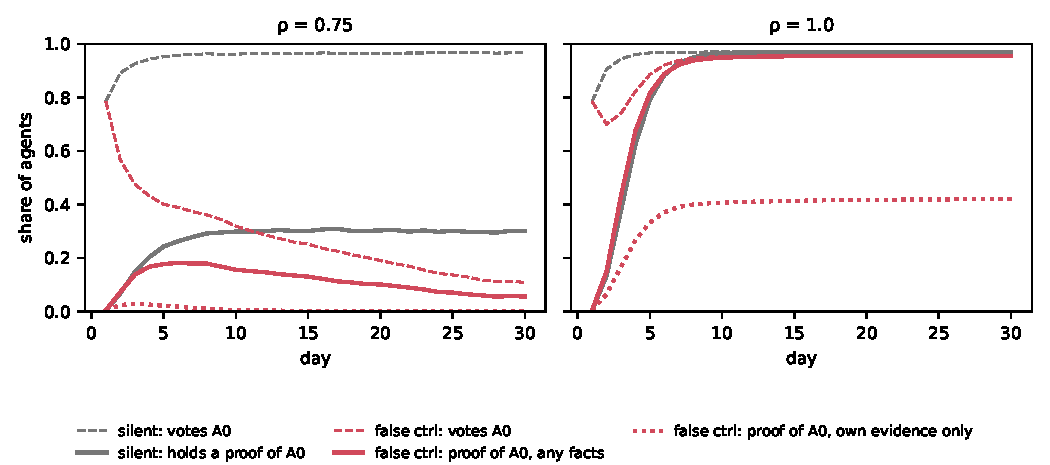
\includegraphics[width=0.95\linewidth]{figures/fig_proof_time.pdf}
\caption{Share of agents voting A0 (dashed) and holding a proof of A0 (solid), silent
against false controller. Dotted: proof from the agents' own original evidence only.
Base rule, $q = 6$, $q_c = 12$, $b = 3$.}
\label{fig:proof}
\end{figure}

\paragraph{Why memory decides.} Figure~\ref{fig:proof} shows the mechanism. With
forgetting, a proof must be reassembled continually; while the false controller fills
the board with A2 evidence, the agents' proof decays (own-evidence proofs fall to
zero) and the A0 vote follows. With full memory the opposite happens: agents
accumulate facts, including the controller's A2 facts. \textbf{Those facts are true},
so together with the agents' evidence they complete proofs of A0: on day 30, 95.6\% of
agents hold a proof of A0, but only 42\% from their own evidence. The rest are proofs
the false controller helped build. Every fact a truthful controller posts eventually
narrows the possible worlds toward the real one, and with full memory nothing is lost.

\section{The controller senses the swarm accurately}

Each night the controller estimates the share of agents backing its target from the
$n \le q_c$ agent posts it reads:
\begin{equation}\label{eq:vhat}
\hat v = \frac{1}{n}\sum_{i=1}^{n} \mathbb{1}\{\text{author of post } i \text{ voted for the target}\},
\end{equation}
and stays silent when $\hat v \ge 0.75$. Each agent posts at most once a day, so the
day's board is nearly a census of votes and $\hat v$ is an unbiased sample of it.

\begin{figure}[H]
\centering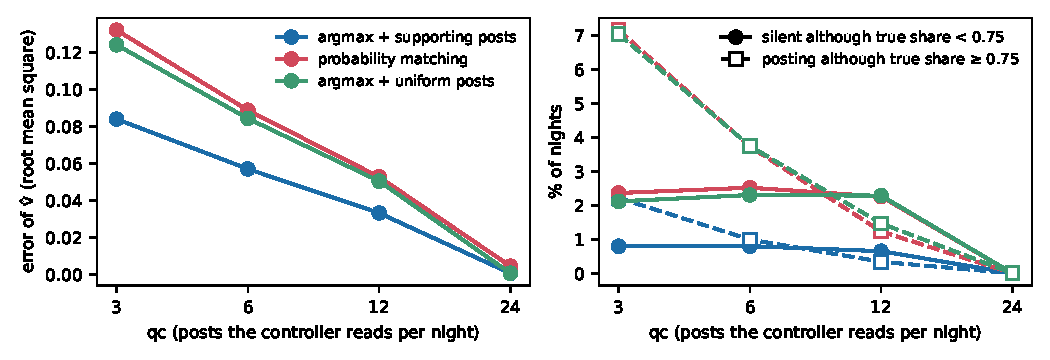
\includegraphics[width=0.95\linewidth]{figures/fig_sensing.pdf}
\caption{Left: error of $\hat v$ against the true share of the 24 agents. Right: gate
mistakes. Mean over arms, $q$, $b$, $\rho$; task003-symmetric.}
\label{fig:sensing}
\end{figure}

\begin{itemize}\itemsep1pt
\item \textbf{No bias}: $\hat v$ minus the true share averages within $\pm 0.0005$.
\item \textbf{The error shrinks with $q_c$} as random sampling predicts, and vanishes at
  $q_c = 24$, where the controller reads every post (Figure~\ref{fig:sensing}, left).
\item \textbf{Gate mistakes are rare} (right panel): under 2\% of nights at $q_c \ge 12$.
  They grow at $q_c = 3$, where the gate needs all 3 posts to agree.
\item \textbf{Abstention does not distort it}: agents almost never abstain (0.1\% of
  agent-days, probability matching only).
\end{itemize}
So in this setup, \textbf{a controller fails because of what it posts, not what it
sees.}

\section{Helping the truth is not helping agents assemble their own proof}

The truth controller stays silent when its sample of the board already proves A0
(\texttt{silent\_when\_target\_proved}). We reran all its cells with that rule off and
compared, episode by episode, two measures: an agent holds a proof of A0 (i)~from any
facts it remembers; (ii)~from its own original evidence only.

\begin{table}[H]
\centering\small
\caption{Rule off minus rule on, day 30, truth controller, mean over $q$, $q_c$, $b$. ``Rule fires'': share of nights the controller sees A0 proved; ``posts despite proof'': share of nights it posts although A0 is proved.}
\label{tab:rule}
\begin{tabular}{lcccc}
\toprule
agent rule, $\rho$ & rule fires (on) & posts despite proof (off) & $\Delta$ proof, any facts & $\Delta$ proof, own evidence \\
\midrule
base, 0.75 & 29\% & 0.3\% & +0.006 & $-$0.012 \\
base, 1.0 & 32\% & 0.3\% & 0.000 & $-$0.029 \\
prob.\ matching, 0.75 & 34\% & 2.3\% & +0.016 & $-$0.044 \\
prob.\ matching, 1.0 & 31\% & 0.8\% & 0.000 & $-$0.057 \\
\bottomrule
\end{tabular}
\end{table}

\begin{figure}[H]
\centering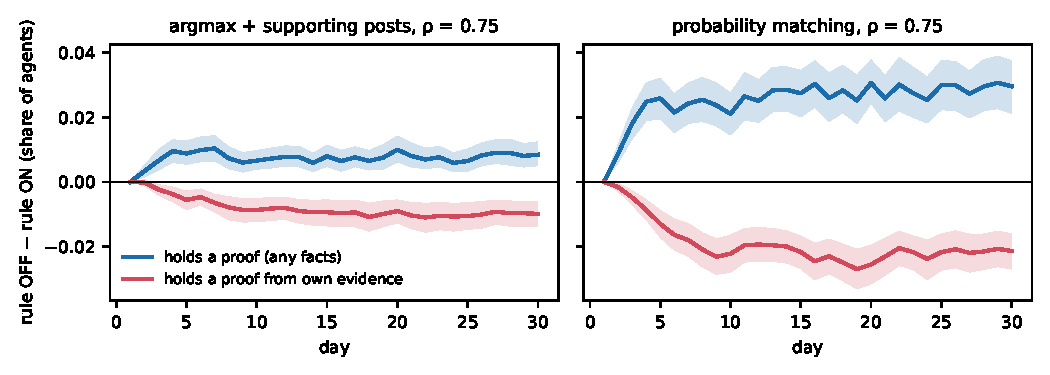
\includegraphics[width=0.95\linewidth]{figures/fig_own_proof.pdf}
\caption{Rule off minus rule on, over days: proof from any facts (blue) and from own
evidence (red). $q = 6$, $q_c = 12$, $b = 1$, $\rho = 0.75$.}
\label{fig:ownproof}
\end{figure}

\begin{itemize}\itemsep1pt
\item \textbf{The vote gate already does most of the stopping}: the rule fires on about
  30\% of nights, yet with it off the controller posts on at most 2\% of nights, because
  by then 75\% of the posts it reads already vote A0 (Table~\ref{tab:rule}).
\item \textbf{The few extra posts pull the two measures apart} (Figure~\ref{fig:ownproof}):
  more agents hold a proof, but fewer hold one from their own evidence.
\item \textbf{Mechanism: posting, not reading.} Controller posts are at most 1.5\% of what
  agents read. But an agent passes on one fact a day, and a controller fact it read on
  an earlier day now competes with its original evidence for that slot (Table~\ref{tab:sub}).
  The original evidence circulates less, so fewer agents assemble it into a proof.
\item Figure~\ref{fig:proof} shows the same split for the false controller, much
  larger: at $\rho = 1$, 95.6\% of agents hold a proof of A0 but only 42\% from their
  own evidence.
\end{itemize}

\begin{table}[H]
\centering\small
\caption{What agents read and post, rule on vs off. Truth controller, probability
matching, $\rho = 0.75$, $q = 6$, $q_c = 12$, $b = 3$, all days.}
\label{tab:sub}
\begin{tabular}{lcccc}
\toprule
rule & reads from controller & posts of own evidence & posts of pool facts & own facts held \\
\midrule
on & 1.34\% & 78.3\% & 27.3\% & 5.81 \\
off & 1.50\% & 76.1\% & 29.3\% & 5.67 \\
\bottomrule
\end{tabular}
\end{table}

\paragraph{Caveats.} One world (task\_003), 24 agents, exact-Bayesian agents; numbers
are means over 1,000 episodes per cell. Full analysis, code and every table:
\texttt{analysis/task003\_llm\_free/sim1\_analysis/} (reports Q0--Q6).

\end{document}
